\documentclass[14pt]{beamer}
\usetheme{Boadilla}

\usepackage[utf8]{inputenc}
\usepackage[T1]{fontenc}
\usepackage[portuguese]{babel}
\usepackage{booktabs}
\renewcommand{\arraystretch}{1.2}

\title[eProfile]{Um Modelo para Gerenciamento de Perfis de Entidades Através de Inferência em Trilhas}
\author{André Wagner}
\institute[UNISINOS]{
  Programa de Pós-Graduação em Computação Aplicada \\
  Unidade Acadêmica de Pesquisa e Pós-Graduação \\
  Universidade do Vale do Rio dos Sinos (UNISINOS) \\
  \texttt{andre.nho@gmail.com}
}

\begin{document}

%%%

\begin{frame}[plain]
  \titlepage
\end{frame}

%%%

\begin{frame}
  \frametitle{Computação Ubíqua}
  \begin{itemize}
    \item Tendências da computação
    \begin{itemize}
      \item Computadores cada vez menores e mais rápidos
      \item Componentes cada vez mais baratos
      \item Acesso a redes \item{wireless} cada vez mais disponível
    \end{itemize}
    \item Serviços computacionais disponíveis a todo momento em qualquer lugar
    \item Tecnologia Calma
    \begin{itemize}
      \item Problema: sobrecarga de informações para o usuário
      \item Solução: sistemas minimamente intrusivos
      \item ``Periferia'' da atenção do usuário
      \item Exemplo: motor de carro
    \end{itemize}
  \end{itemize}
\end{frame}

%%%%%

\begin{frame}
  \frametitle{Contexto}
  \begin{itemize}
    \item Para que um sistema seja minimamente intrusivo
    \begin{itemize}
      \item Conhecer o usuário
      \item Conhecer os arredores do usuário
      \item Adaptar-se a esta informação
    \end{itemize}
    \item {\bf O que é contexto?}
    \begin{itemize}
      \item ``Contexto é qualquer informação que possa ser usada para 
      caracterizar a situação de uma entidade. Uma entidade é uma pessoa, 
      local ou objeto que seja considerada relevante para a interação entre 
      um usuário e uma aplicação, incluíndo os próprios usuário e aplicação.'' (Dey, 2001)
    \end{itemize}
  \end{itemize}
\end{frame}
    
%%%%%

\begin{frame}
  \frametitle{Trilhas}
  \begin{itemize}
    \item Contexto é composto apenas pelo momento atual
    \item A capacidade de uma aplicação compreender o contexto de uma entidade pode ser ampliada através da análise dos históricos.
    \item Uma \textbf{trilha} é o histórico de contextos visitados por uma entidade, e das ações realizadas pela entidade dentro do contexto
  \end{itemize}
\end{frame}
    
%%%%%

\begin{frame}
  \frametitle{Perfis}
    \begin{itemize}
      \item \textbf{Perfis} são essenciais na descoberta de informações pertinentes aos usuários que possam ser utilizadas na construção de um contexto.
      \item Um \textbf{perfil de usuário} é o conjunto de dados no qual uma aplicação armazena seu conhecimento a respeito de um usuário. 
      \item Os perfis de usuário são salvos em um formato chamado \textbf{modelo de usuário}.
      \item Este trabalho usa o conceito de \textbf{entidade} ao invés de usuário.
    \end{itemize}
\end{frame}
    
%%%%%

\begin{frame}
  \frametitle{Interoperabilidade}
  \textbf{Interoperabilidade} é a capacidade de dois ou mais sistemas ou componentes trocarem informações e utilizar a informação que foi trocada.
  \begin{itemize}
    \item Modelos de Interoperabilidade
    \begin{description}
      \item[Sintática:] diferenças entre os modelos de usuário são resolvidos em nível de aplicação.
      \item[Semântica:] diferenças entre os modelos são resolvidos em nível de conhecimento.
    \end{description}
  \end{itemize}
\end{frame}
    
%%%%%%%%%%%%%%%%%%%%%%

\begin{frame}[shrink=10]{Trabalhos Relacionados - PeLeP}

  \begin{center}
    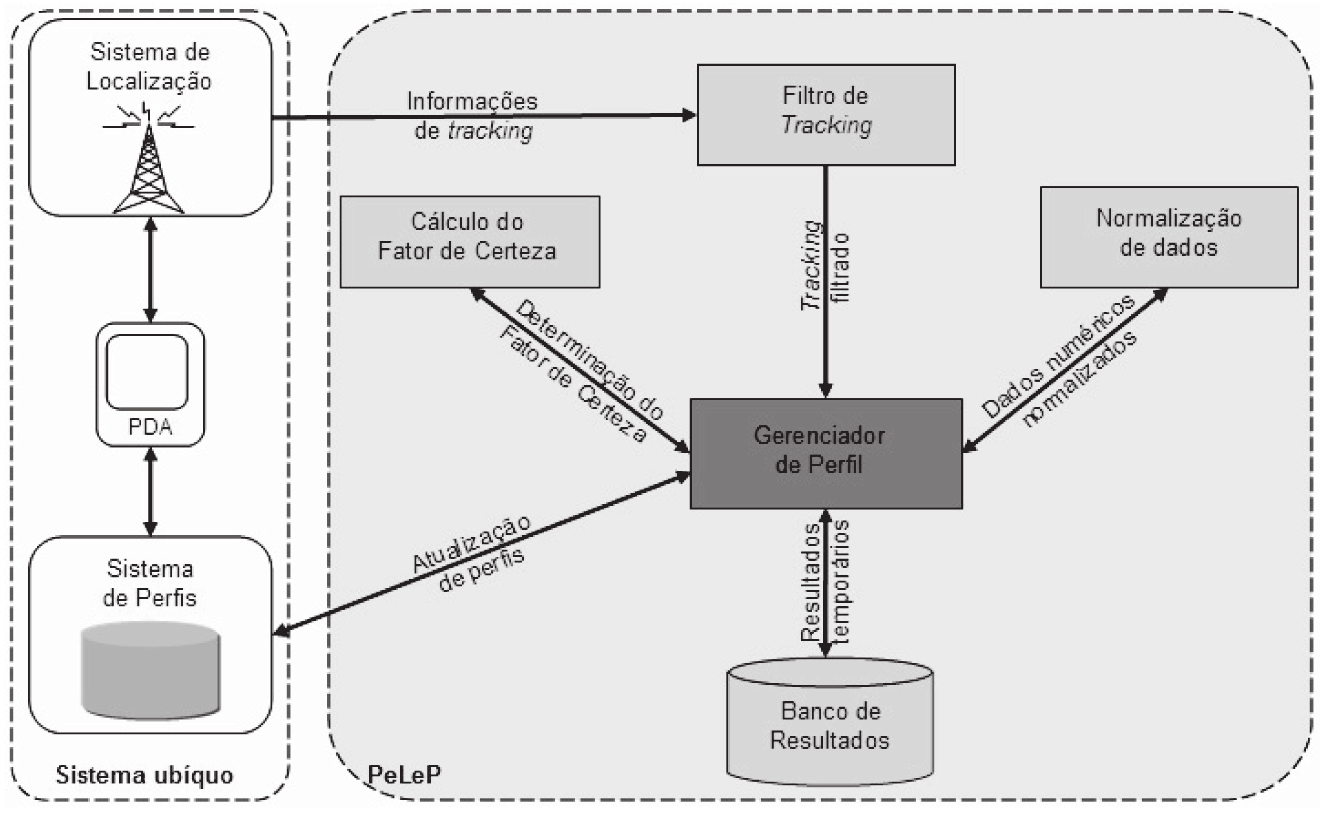
\includegraphics[width=0.5\textwidth]{../imagens/pelep1.png}
  \end{center}

  \begin{itemize}
    \item Suporta o aperfeiçoamento automático do perfil do aprendiz em ambientes de educação ubíqua.
    \item Usa o histórico dos aprendizes nos contextos de um ambiente ubíquo para atualização dos perfis.
    \item O perfil do aprendiz no modelo é refinado e enriquecido através de inferências.
    \item As inferências são baseadas na mobilidade do aprendiz e no monitoramento das tarefas que ele executa nos contextos de um ambiente de educação ubíqua.
  \end{itemize}

\end{frame}

%%%%%%%%%%%%%%%%%%%%%%

\begin{frame}{Trabalhos Relacionados - Chellouche et al}

  \begin{center}
    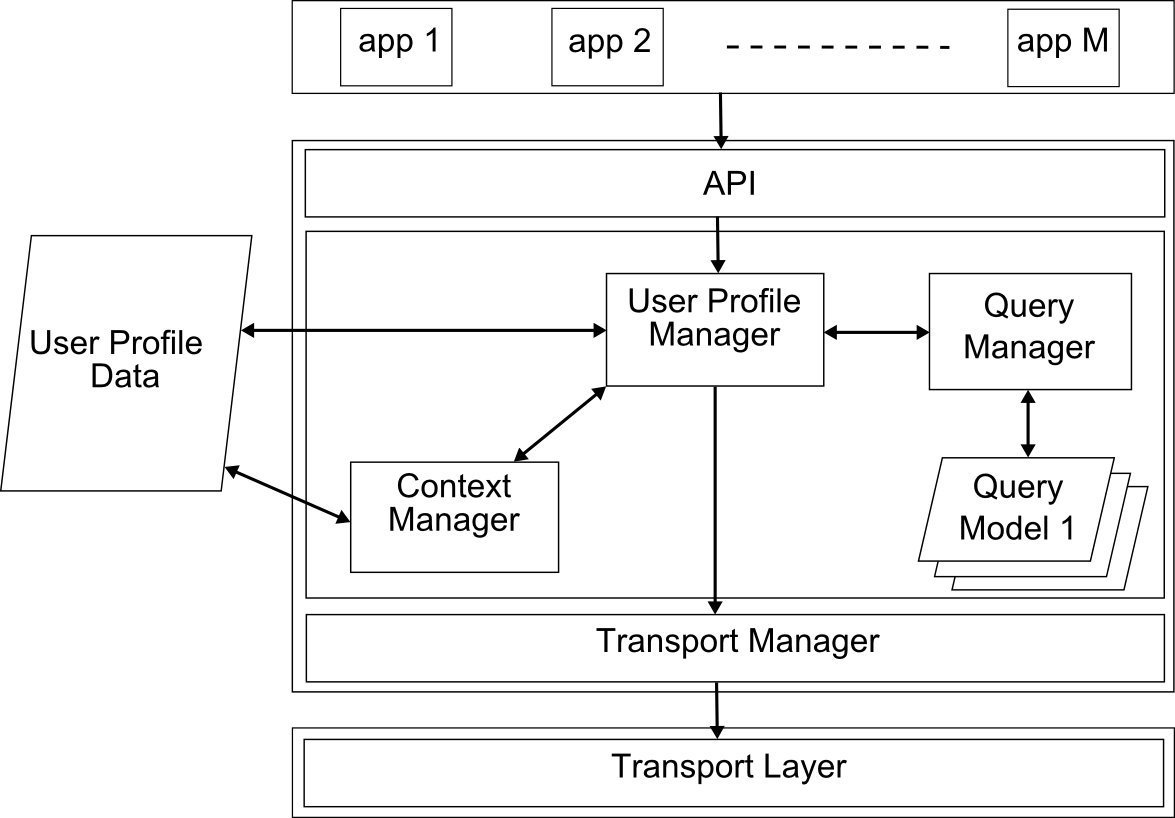
\includegraphics[width=0.4\textwidth]{../imagens/chellouche1.png}
  \end{center}

  \begin{itemize}
    \item \emph{Middleware} que pode ser usado por diferentes aplicativos como um servidor central de perfis.
    \item Voltado para aplicações móveis.
    \item Não permite que os aplicativos criem novos campos nem definam as regras para atualização dos campos existentes.
  \end{itemize}

\end{frame}

%%%%%%%%%%%%%%%%%%%%%%

\begin{frame}{Trabalhos Relacionados - UUCM}

  \begin{columns}
    \begin{column}{0.6\textwidth}
      \begin{itemize}
        \item Pode ser utilizado para modelar as características de um usuário e seu contexto em ambientes de personalização inter-sistemas.
        \item Requer que os sistemas que utilizam este modelo concordem em uma ontologia básica.
        \item Utiliza a ideia de \emph{passaporte}, onde o usuário leva seu perfil consigo.
      \end{itemize}
    \end{column}
    \begin{column}{0.4\textwidth}
      \begin{center}
        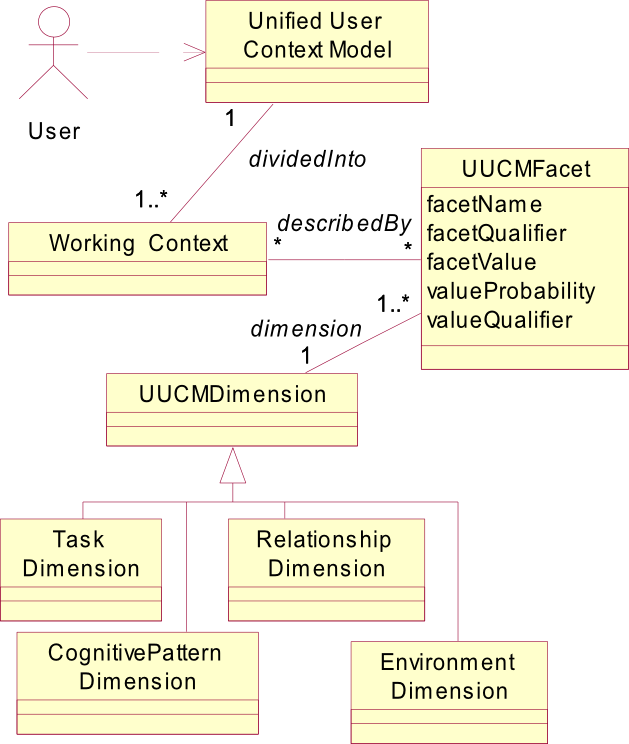
\includegraphics[width=1\textwidth]{../imagens/niederee1.png}
      \end{center}
    \end{column}
  \end{columns}

\end{frame}

%%%%%%%%%%%%%%%%%%%%%%

\begin{frame}{Comparação entre os trabalhos apresentados}

\begin{table}\centering\footnotesize
  \begin{tabular*}{1\textwidth}{@{}lllllll@{}}
    \toprule
                              & PeLeP    & Chellouche et al   & UUCM \\
    \midrule
    Interoperabilidade        & Não      & Sintática          & Sintática \\
    Perfis dinâmicos          & Sim      & Sim                & Sim \\
    Armazenamento             & Servidor & Servidor           & Cliente \\
    Sensibilidade a contexto  & Sim      & Sim                & Sim \\
    Utiliza trilhas           & Parcial  & Não                & Não \\
    Domínio                   & Educação & Serviços multimídia & Genérico \\
    \bottomrule
  \end{tabular*}
  \caption{Comparação entre os trabalhos apresentados}
  \label{tab:comparacao}
\end{table}

\end{frame}

%%%%%

\begin{frame}
  \frametitle{Problema de Pesquisa}
  \begin{itemize}
    \item O sistema deve obter a intenção do usuário
    \item Para isso, ele precisa conhecer o usuário, seu contexto e histórico
    \item Alguns trabalhos recentes buscam obter seu perfil a partir da trilha
    \item Mas todos em um domínio específico (ex. educação, comércio)
    \item Desafio: um modelo que trabalhe em um domínio genérico
  \end{itemize}
\end{frame}

%%%%%

\begin{frame}
  \frametitle{eProfile}
\textbf{eProfile}: um \textcolor{blue}{gerenciador de perfis} de \textcolor{blue}{domínio genérico} voltado para \textcolor{blue}{ambientes distribuídos}, com \textcolor{blue}{interoperabilidade inter-sistemas}, que \textcolor{blue}{infere dados de perfil} através da \textcolor{blue}{análise das trilhas} de uma entidade (disponibilizadas por um gerenciador de trilhas), seguindo \textcolor{blue}{regras definidas pelas entidades}, e \textcolor{blue}{disponibiliza os dados} inferidos para serem utilizados pelas aplicações.
\end{frame}

%%%%%

\begin{frame}
  \frametitle{Modelo do eProfile}
\begin{figure}
  \centering
\includegraphics[width=0.7\textwidth]{../imagens/modelobasico.png}
  \caption{Modelo básico do eProfile}
\end{figure}
As setas representam o fluxo dos dados.
\end{frame}


%%%%%

\begin{frame}
  \frametitle{Modelo do eProfile}
\begin{figure}
  \centering
\includegraphics[width=0.7\textwidth]{../imagens/modelo2.png}
  \caption{eProfile conectado a mais de um gerenciador de trilhas}
\end{figure}
\end{frame}

%%%%%

\begin{frame}
  \frametitle{Modelo do eProfile}
\begin{figure}
  \centering
\includegraphics[width=0.9\textwidth]{../imagens/modelo.png}
  \caption{Modelo simplificado do eProfile}
\end{figure}

\end{frame}

%%%%%

\begin{frame}
  \frametitle{Ontologias}
  \begin{itemize}
    \item Extensível
    \item Linguagem utilizada: OWL (extensão de XML/RDF)
  \end{itemize}
  Ontologias do eProfile
  \begin{itemize}
    \item eOntoTrail: representação de trilhas
    \item eOntoProfile: representação de perfis
  \end{itemize}
\end{frame}

%%%%%

\begin{frame}
  \frametitle{Ontologia de Trilha}
\begin{figure}
  \centering
\includegraphics[width=1\textwidth]{../imagens/ont_trilha.png}
  \caption{Ontologia de Trilha do eProfile}
\end{figure}
  
\end{frame}

%%%%%

\begin{frame}
  \frametitle{Ontologia de Perfis}
\begin{figure}
  \centering
\includegraphics[width=0.8\textwidth]{../imagens/ont_perfil2.png}
  \caption{Ontologia de Perfil do eProfile}
\end{figure}

\end{frame}

%%%%%

\begin{frame}
  \frametitle{Regras}
  \begin{itemize}
    \item Regras em SPARQL (consulta) ou SWRL (lógica)
    \item Um regra possui as seguintes informações:
    \begin{itemize}
      \item Nome
      \item Campo de perfil
      \item Regra
      \item Atualização (sobrescrito/fórmula)
      \item Freqüência de atualização
      \item Validade
    \end{itemize}
  \end{itemize}
\end{frame}

%%%%%

\begin{frame}
  \frametitle{Situação Atual}
  \begin{itemize}
    \item Proposta aprovada
    \item Protótipo básico implementado
    \item Um cenário criado e implementado
    \item Artigo submetido ao WSCAD (Simpósio de Sistemas Computacionais)
  \end{itemize}
\end{frame}

%%%%%% 

\begin{frame}
  \frametitle{Implementação do Protótipo}
  \begin{itemize}
    \item Desenvolvimento: Python (substitui Java)
    \item Banco de dados: SQLite
    \item Aplicação de regras: Pellet (substitui HermiT)
    \item Gerenciador de trilhas: próprio / eTrail (?)
  \end{itemize}
\end{frame}

%%%%%

\begin{frame}
  \frametitle{Validação}
  \begin{itemize}
    \item O eProfile é uma proposta de infraestrutura.
    \item Propostas deste tipo são avaliadas construindo aplicações que a utilizem e então avaliando-as, obtendo uma avaliação indireta do modelo.
    \item Cenários tem sido usados na avaliação indireta de modelos sensíveis a contexto e ubíquos.
  \end{itemize}
\end{frame}

%%%%%

\begin{frame}
  \frametitle{Validação}
  \begin{itemize}
    \item Avaliação da proposta -- duas perspectivas:
    \begin{itemize}
      \item {\bf Funcionalidade:} o protótipo é funcional e atende o modelo proposto?
      \item {\bf Cenário:} criação e implementação de dois cenários.
    \end{itemize}
  \end{itemize}
  \begin{itemize}
    \item Cenários:
    \begin{enumerate}
      \item Educação ubíqua: geração de perfis de estudantes através da avaliação de trilhas (simples);
      \item Confiança: cálculo de confiança de entidades baseado na análise de transações comerciais.
    \end{enumerate}
  \end{itemize}

\end{frame}

%%%%%

\begin{frame}
  \frametitle{Obrigado!}
  Perguntas?
\end{frame}

\end{document}
